\RequirePackage{plautopatch}
\documentclass[twocolumn]{article}
\usepackage{amsmath}
\usepackage{amssymb}
\usepackage{booktabs}
\usepackage{CJK}
\usepackage{courier}
\usepackage{helvet}
\usepackage{latexsym}
\usepackage{marvosym}
\usepackage{multirow}
\usepackage{rotating}
\usepackage{setspace}
\usepackage{stmaryrd}
\usepackage{tabularx}
\usepackage{textcomp}
\usepackage{times}
\usepackage{url}
\usepackage{wasysym}
\usepackage{here}
\usepackage{ascmac}
\usepackage{setspace}
\spacing{0.95}
\usepackage{breakcites}
\usepackage{fancyhdr}
\usepackage{graphicx}
\usepackage{xurl}
\usepackage{float}
\usepackage{subcaption}
\usepackage{caption}
\usepackage{tabularx}
\usepackage{fdsymbol}
\usepackage{enumitem}
\setlength{\textfloatsep}{0pt plus 0pt minus 0pt}
\setlength{\floatsep}{0pt plus 0pt minus 0pt}
\setlength{\intextsep}{0pt plus 0pt minus 0pt}
\setlength{\dbltextfloatsep}{0pt plus 0pt minus 0pt}
\setlength{\dblfloatsep}{0pt plus 0pt minus 0pt}
\setlength{\abovecaptionskip}{5pt}  % space above caption
\setlength{\belowcaptionskip}{5pt}   % space below caption (optional)
\setlength{\itemsep}{0pt plus 0pt minus 0pt}
\setlist[itemize]{noitemsep,topsep=0pt}
\setlist{nolistsep}
\setlist{nosep}
\usepackage[compact]{titlesec}
\titlespacing{\section}{1pt}{2ex}{1ex}
\titlespacing{\subsection}{1pt}{1ex}{1ex}
\titlespacing{\subsubsection}{1pt}{1ex}{1ex}
\setlength{\parskip}{0cm}
\setlength{\parindent}{0cm}
% \renewcommand*{\@seccntformat}[1]{\csname the#1\endcsname\hspace{0mm}}
\newcommand{\textdaggertriple}{\textdagger\textdagger\textdagger}
\newcommand{\textdaggerdouble}{\textdagger\textdagger}
\fancypagestyle{firstpage}
{
    \fancyhead[L]{}
    \fancyhead[C]{\Large 言語獲得と理解研究会報告(Summer 2025)}    
    \fancyhead[R]{}
}

\setlength{\oddsidemargin}{-3.4mm}
\setlength{\evensidemargin}{-3.4mm}
\setlength{\topmargin}{1.3mm}
\setlength{\headheight}{0mm}
\setlength{\headsep}{-1mm}
\setlength{\textwidth}{18cm}
\setlength{\textheight}{24.6cm}
\setlength{\columnsep}{0.8cm}
\setlength{\leftmargin}{-0.5cm}
\setlength{\itemsep}{0cm}

\baselineskip=0.9\baselineskip
\abovedisplayskip=0.8\abovedisplayskip
\belowdisplayskip=0.8\belowdisplayskip
\abovedisplayshortskip=0.8\abovedisplayshortskip
\belowdisplayshortskip=0.8\belowdisplayshortskip

\def\AND{\hskip 2em plus 40fil}

\newcounter{ex}
\newcommand{\itemex}{\refstepcounter{ex}\item[\textmd{\textrm{(\theex)}}]}
\renewcommand{\indent}{\hspace*{2em}}
\def\ex#1{
\begin{description}
 \itemex #1
\end{description}
}
\title{\textbf{Impact of Bucketing with BERT Embeddings on Model Performance across Training Set Sizes}}
\author{
    \begin{center}
        \begin{tabular}{ccc}
            \multicolumn{3}{c}{
            \begin{tabular}{ccc}
            \Large{Christian Harjuno\textdagger} & 
            \Large{Victor Silaa \textdagger} & 
            \Large{Yoko Nakajima\textdagger}
            \end{tabular}}\\[5pt]
            \multicolumn{3}{c}{
            \begin{tabular}{cc}
              \Large{Tomoyosi Akiba\textdaggerdbl} & \Large{Hirotoshi Honma\textdaggerdbl} 
            \end{tabular}} \\[5pt]
            \multicolumn{3}{c}{\textdagger\space Department of Computer Science, Kushiro College of Technology}\\
            \multicolumn{3}{c}{\texttt{p234071@kushiro.kosen-ac.jp, \{silaa,yoko,honma\}@kushiro-ct.ac.jp}}\\[2pt]
            \multicolumn{3}{c}{\textdaggerdbl\space Department of Computer Science and Engineering, Toyohashi University of Technology}\\
            \multicolumn{3}{c}{\texttt{akiba@cs.tut.ac.jp}}\\
            [4pt]
            \multicolumn{3}{c}{}\\[-8pt]
            \multicolumn{3}{c}{\textbf{Abstract}}\\
            \multicolumn{3}{p{6.4in}}{\normalsize
                \hspace*{1em} We investigate a semantic bucketing strategy based on BERT embeddings to improve overall model generalization performance on scarce data. Samples are grouped by semantic similarity rather than structural similarity, such as length, and evaluated across varying training dataset sizes. Fine-tuned model performance is evaluated using accuracy, precision, recall, and loss. The results are then compared to a model trained on randomly sampled data. Our experiments show that bucketing consistently yields better metrics on smaller dataset sizes yet reveals higher losses on slightly larger data sizes, suggesting less confident probability estimates.}
        \end{tabular}
    \end{center}
}
\date{}
\begin{document}
\maketitle
\section{Introduction}
\thispagestyle{firstpage}
\indent Pre-trained language representation models, such as BERT, have influenced natural language processing by capturing contextual relationships across massive texts. However, despite their broad linguistic knowledge, these models must be fine-tuned on task-specific datasets to achieve strong downstream performance \cite{DBLP:journals/corr/abs-1810-04805}. The effectiveness of fine-tuning depends heavily on the quality of the training data: datasets must be sufficiently large, balanced across classes, and representative of diverse edge cases to support generalization \cite{zhang2024textbfonlyifrevealingdecisiveeffectinstruction}. This study explores the effects of embedding-based semantic bucketing on model training efficiency. By partitioning datasets using token embeddings rather than token length, we aim to produce buckets that are more coherent in meaning rather than size. We investigate whether sub-sampling bucketed data, compared against randomized sampling, can improve model performance under varying dataset sizes.

\section{Related Studies}
\indent Improving the representation of all edge cases and balancing the training data is critical when fine-tuning pre-trained encoders. One well-established method is \textit{stratified sampling}, which preserves the label distribution across subsets and prevents the overrepresentation of classes. This has been shown to enhance generalization, particularly for minority categories~\cite{merrillees2021stratifiedsamplingextrememultilabel}.

\indent Beyond label-aware sampling, researchers have also explored \textit{bucketing strategies} to manage input variability. A common approach is bucketing by sequence length, which reduces variance in input size and stabilizes training dynamics~\cite{dao2024transformers}. However, Qu, Tu, and Bao (2024) show that length-based chunking yields high topic entropy and low completeness scores, indicating that such buckets mix semantically unrelated material \cite{QuTuBao2024}.

\indent To address this limitation, \textit{embedding-based clustering} has been proposed. Petukhova et al.~\cite{petukhova2025text} show that grouping samples according to sentence embeddings yields semantically coherent clusters, improving coverage of diverse semantic phenomena during fine-tuning. Although less explored than length-based bucketing, this line of work suggests that embedding-driven partitioning may improve robustness in semantically diverse domains, such as social media text.

\indent Based on these previous studies, our study examines if creating buckets of semantically similar samples before sampling evenly across buckets improves the fine-tuned model's generalization performance on smaller dataset sizes. While previous work focuses on comparing cluster quality across different models and bucketing algorithms, not much attention has been given to the effects of these clusters on model performance when only a small amount of data is available. Randomly sampling subsets from a semantically diverse dataset can introduce semantic bias, as some regions may be underrepresented, which potentially harms overall model generalization, particularly when sampled subsets are small\cite{shah-etal-2020-predictive}. Our study aims to address this gap by analyzing whether using embedding-based bucketing to create semantically balanced datasets reduces the amount of data needed to train a well-performing model. The model trained on bucketed data is compared with a model trained on randomly sampled data with varying set sizes. Both models are compared through classification metrics and evaluation loss.

\section{Proposed Solution}\label{proposedsolution}
\indent To mitigate semantic bias in low-sample environments, we propose an embedding-based bucketing strategy to improve BERT fine-tuning on datasets with high semantic variability. First, we convert each text sample into a vector representation using pre-trained BERT embeddings. Next, we reduce the embeddings using UMAP and scale them with StandardScaler\footnote{\url{https://scikit-learn.org/stable/modules/generated/sklearn.preprocessing.StandardScaler.html}}. We then cluster the scaled embeddings using HDBSCAN\footnote{\url{https://scikit-learn.org/stable/modules/generated/sklearn.cluster.HDBSCAN.html}} to form buckets of semantically similar examples. During fine-tuning, we sample a fixed number of examples from each bucket with stratified labels using the global (whole dataset) ratio.

\indent This approach is compared against randomized sampling with approximately equal amounts of data. Unlike length-based methods, embedding-based bucketing produces semantically coherent batches, which we hypothesize will preserve semantic diversity within each batch.

\subsection{Dimension Scaling}\label{scaling}

\indent Peterfreund (2021) states that while the 768 dimensions in BERT embeddings allow subtle contextual signals to be captured, such high-dimensional embeddings introduce noise and increase computational complexity for clustering or bucketing tasks. Redundant or irrelevant features in these embeddings can negatively impact clustering performance \cite{peterfreund2021multidimensional}.

\indent To reduce complexity and preserve important semantics, we apply UMAP (Uniform Manifold Approximation and Projection) to project a higher dimension into a smaller dimension size while maintaining important information \cite{mcinnes2018umap}. UMAP can reduce the dimension size while maintaining both local and global relationships.

\indent We observed that directly reducing 768-dimensional embeddings to 2 dimensions does not yield visually distinguishable clusters. However, introducing an intermediate reduction to 50 dimensions before projecting to 2 dimensions produced clearer and better-separated clusters, which will facilitate downstream clustering with algorithms such as HDBSCAN, as shown in Figure~\ref{fig:umap76850}.

\indent The quality of clusters can be further quantified using several metrics. To measure the cohesion of points within clusters and their separation from other clusters, we utilize the Silhouette Score \cite{ROUSSEEUW198753}. The Davies-Bouldin Score is employed to assess the ratio of intra-cluster scatter to inter-cluster separation \cite{davies1979cluster}. Finally, the Calinski-Harabasz Score measures the ratio of between-cluster variance to within-cluster variance \cite{calinski1974dendrite}. Together, these metrics are able to quantify how cohesive and well-separated the buckets are from each other. A well-separated bucket reduces the chances of data points falling near bucket boundaries, which signify poor clustering. 

\indent As shown in Table~\ref{tab:umap_metrics_vertical}, introducing an intermediate reduction to 50 dimensions before projecting to 2 outperforms a direct reduction from 768 to 2 across all clustering metrics. These metrics collectively demonstrate that the intermediate reduction may produce more coherent and better-separated clusters. The resulting clusters obtained via HDBSCAN are visualized in Figure~\ref{fig:hdbscan-visualization}.

\indent As shown in Figure~\ref{fig:hdbscan-visualization}, introducing an intermediate reduction to 50 dimensions results in less noise (highlighted in purple) compared to a direct reduction from 768 to 2 dimensions.

\indent Based on the observations from the UMAP reductions and HDBSCAN clustering, we will adopt the two-step dimensionality reduction approach — first reducing BERT embeddings from 768 to 50 dimensions, followed by a further reduction to 2 dimensions—for all subsequent clustering experiments. 
\begin{figure}[H]
    \centering
    \begin{subfigure}[b]{\linewidth}
        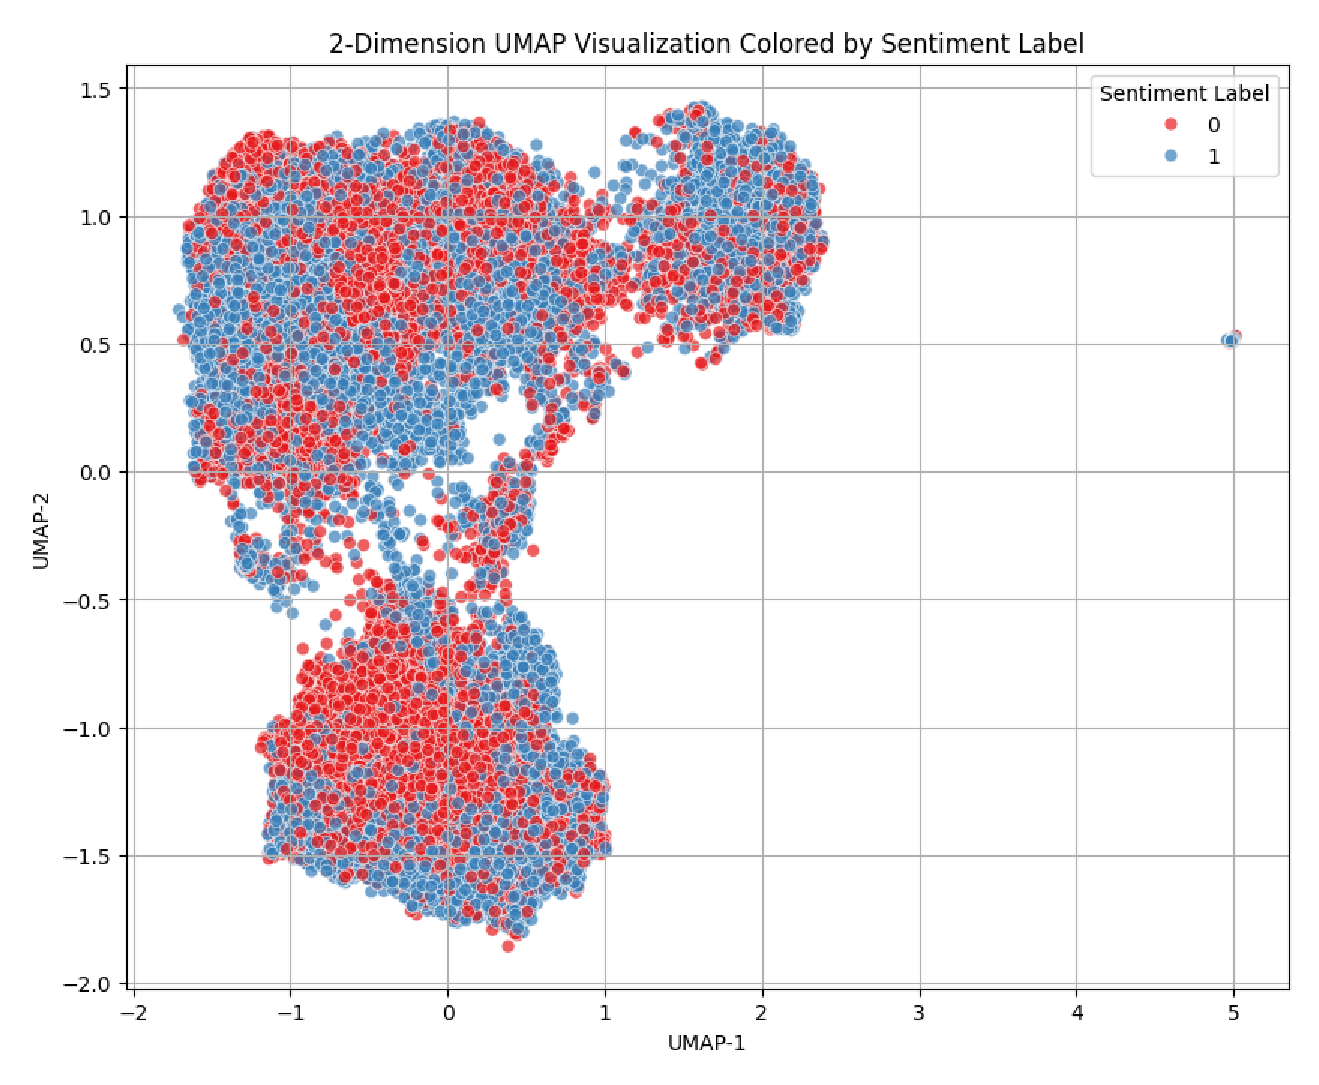
\includegraphics[width=\linewidth]{768-2.eps}
        \caption{UMAP Reduction from 768 to 2}
    \end{subfigure}
    \begin{subfigure}[b]{\linewidth}
        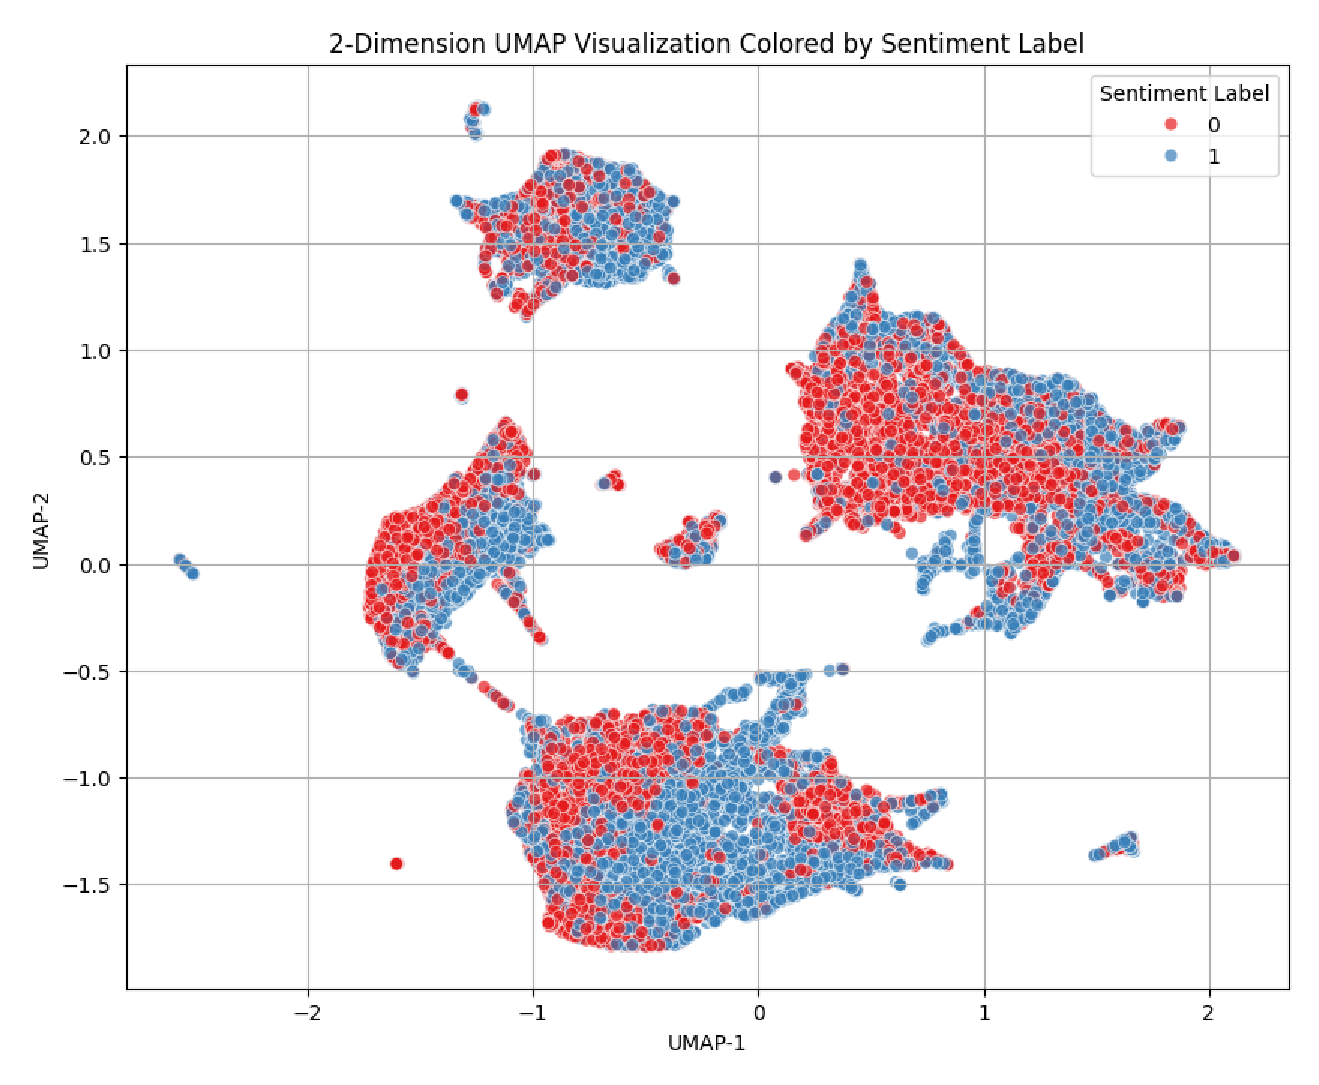
\includegraphics[width=\linewidth]{768-50-2.eps}
        \caption{UMAP Reduction from 768 to 50, then 2}
    \end{subfigure}
    \caption{Comparison of UMAP dimensionality reduction strategies.}
    \label{fig:umap76850}
\end{figure}

This strategy has been shown to potentially produce more semantically coherent clusters, reduce noise, and improve cluster separation, thereby providing a more reliable basis for embedding-based bucketing in downstream fine-tuning tasks. However, the general effectiveness of this strategy is still unclear and needs further testing before it can be fully implemented in the current workflow. 

\subsection{Clustering with HDBSCAN}\label{clusteringwithhdbscan}
\indent Traditional clustering methods often use K-Means to partition vectors into clusters. While K-Means allows specifying a fixed number of clusters, it assumes that clusters are roughly spherical and of similar size \cite{IKOTUN2023178}. However, BERT embeddings have been shown to be anisotropic, occupying a narrow cone in vector space \cite{ethayarajh-2019-contextual}, making K-Means unsuitable for this type of data. 

\indent In contrast, HDBSCAN (Hierarchical Density-Based Spatial Clustering of Applications with Noise) \cite{10.1007/978-3-642-37456-2_14} can identify clusters of arbitrary shapes and dynamically determine the number of clusters based on the data. Additionally, HDBSCAN can handle noise points effectively, leaving them unassigned to any cluster, which is particularly useful for noisy embeddings.

This makes HDBSCAN particularly suitable for creating semantically coherent buckets from BERT embeddings.
\begin{figure}[H]
    \centering
    \begin{subfigure}[b]{\linewidth}
        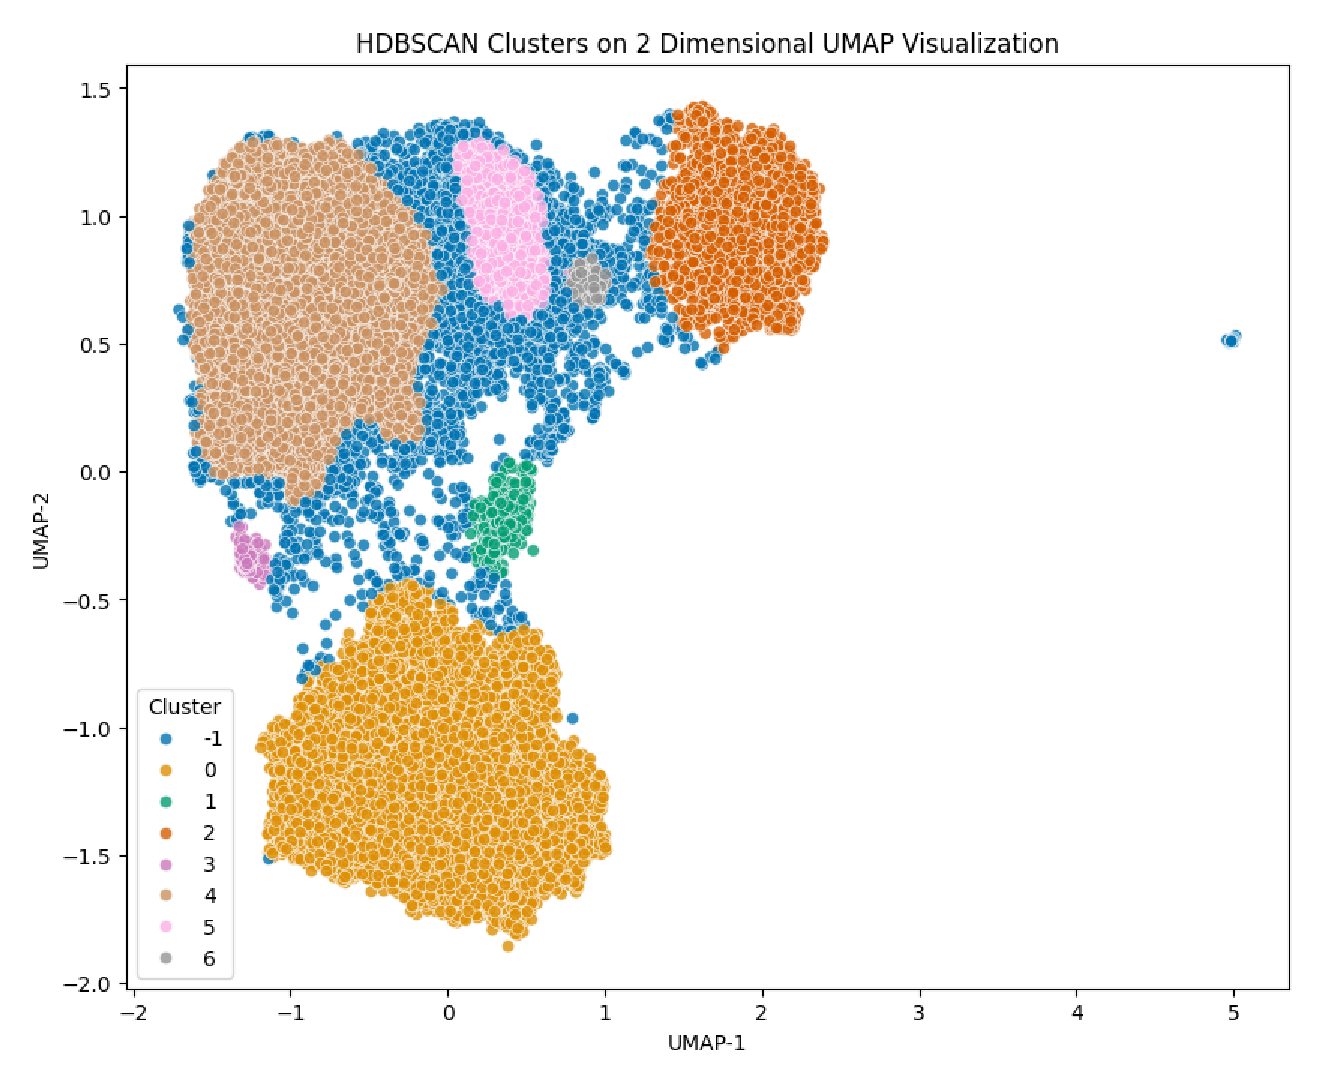
\includegraphics[width=\linewidth]{hdbscan-768-2.eps}
        \caption{HDBSCAN clusters after UMAP reduction from 768 to 2 dimensions}
        \label{fig:hdbscan-visualization-figure1}
    \end{subfigure}
    \begin{subfigure}[b]{\linewidth}
        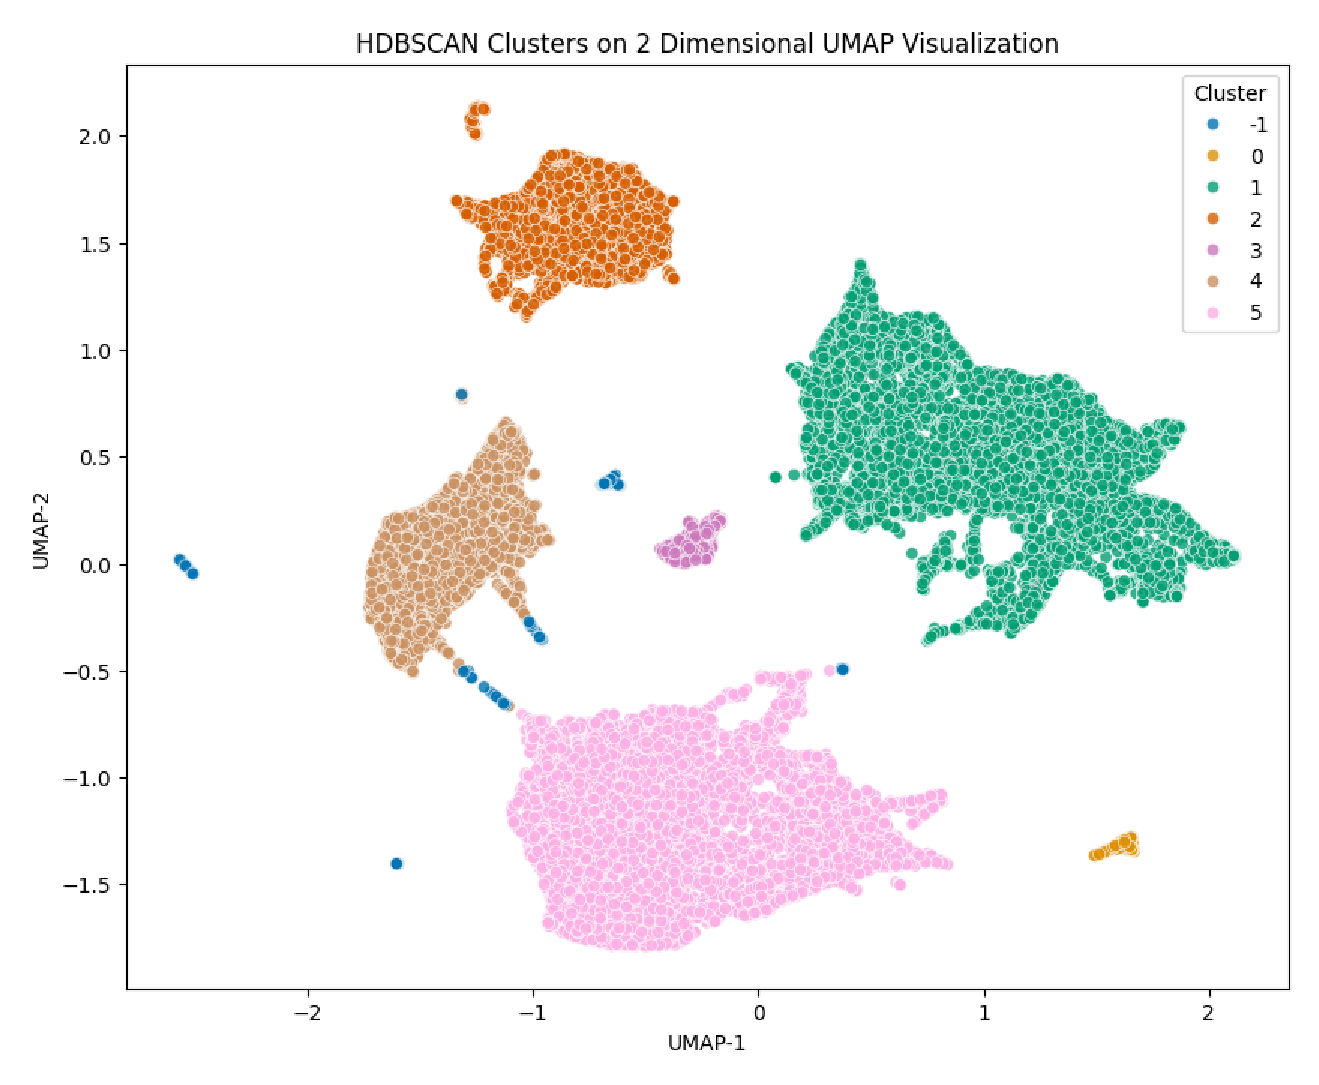
\includegraphics[width=\linewidth]{hdbscan-768-50-2.eps}
        \caption{HDBSCAN clusters after UMAP reduction from 768 to 50, then to 2 dimensions}
        \label{fig:hdbscan-visualization-figure2}
    \end{subfigure}
    \caption{Visualization of HDBSCAN clustering performance under different UMAP reduction strategies}
    \label{fig:hdbscan-visualization}
\end{figure}

\section{Data}\label{data}
\indent A few considerations went into determining which public dataset will be used in this experiment. Having a clean, balanced, and accurate dataset can help in reducing variability, which affects our final results. Datasets such as the Stanford IMDB dataset (stanfordnlp/imdb) \cite{maas-EtAl:2011:ACL-HLT2011} are popular due to their simplicity, cleanliness, and balance. However, the goal of bucketing is to provide the model with a balanced representation of all semantic edge cases in the dataset. If we apply the clustering techniques previously explained in Section \ref{proposedsolution}, we can visualize the clusters as shown in Figure \ref{fig:imdbembeddings}

\begin{table}[H]
  \begin{center}
    \caption{Clustering metrics for different UMAP reduction strategies. Arrows indicate whether higher (\(\uparrow\)) or lower (\(\downarrow\)) values are better.}
    \label{tab:umap_metrics_vertical}
    \resizebox{\linewidth}{!}{%
    \begin{tabular}{lcc}
      \toprule
      \textbf{Metric} & \textbf{768 $\rightarrow$ 50 $\rightarrow$ 2} & \textbf{768 $\rightarrow$ 2} \\
      \midrule
      Silhouette Score (\(\uparrow\)) & 0.5002 & 0.3785 \\
      Davies-Bouldin Score (\(\downarrow\)) & 0.4352 & 0.4817 \\
      Calinski-Harabasz Score (\(\uparrow\)) & 46558.54 & 41264.99 \\
      \bottomrule
    \end{tabular}
    }
  \end{center}
\end{table}


\begin{figure}[H]
    \centering
    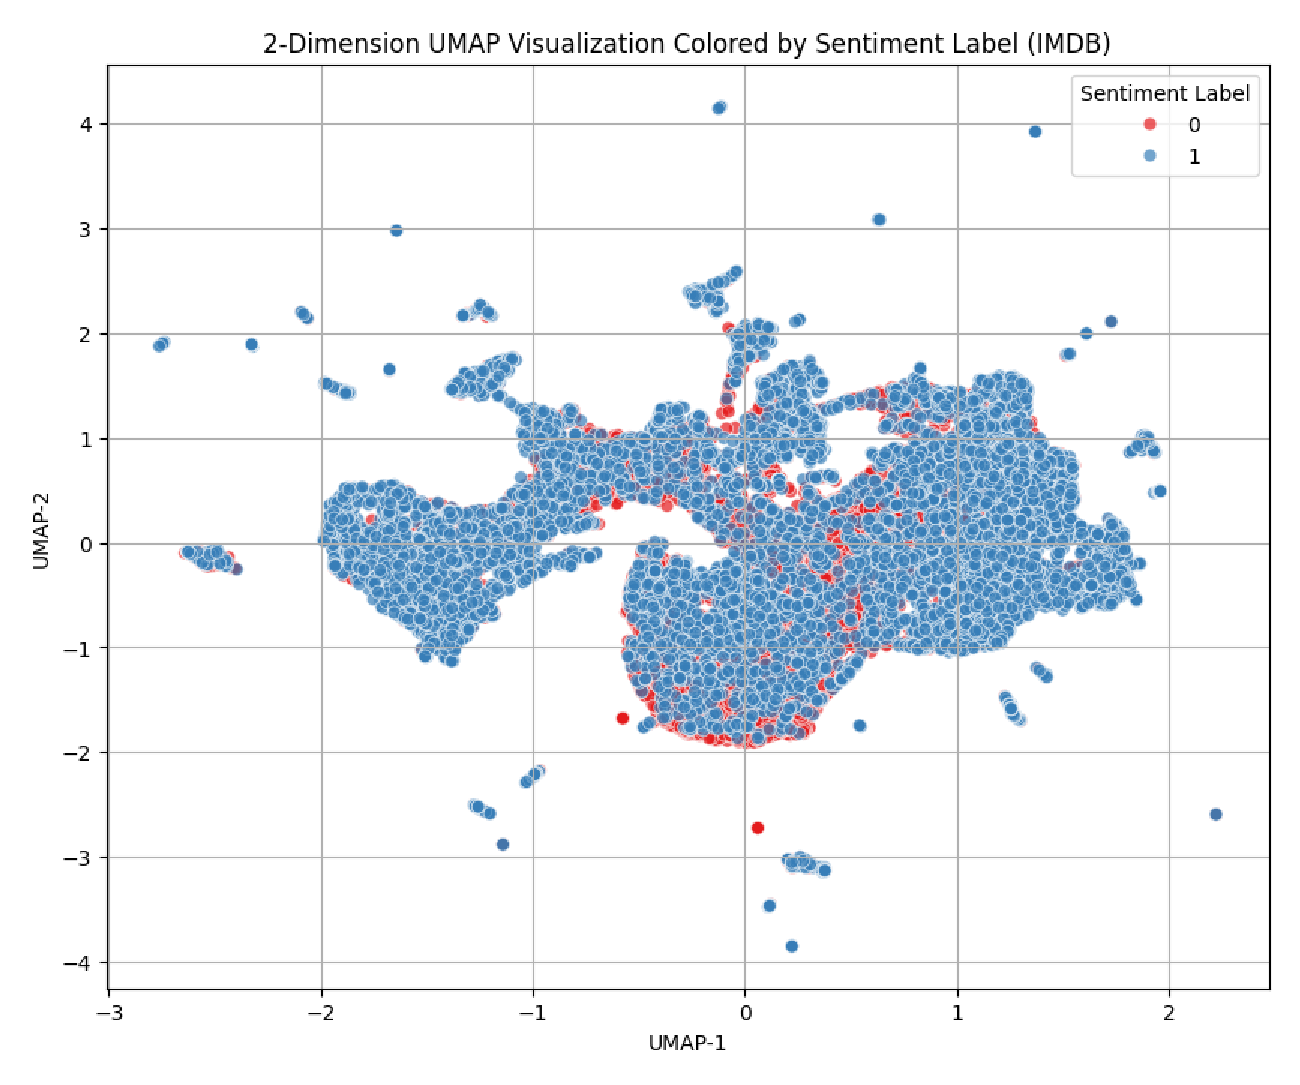
\includegraphics[width=\linewidth]{imdb-embeddings.eps}
    \caption{stanfordnlp/imdb embeddings visualized}\label{fig:imdbembeddings}
\end{figure}

\indent Due to low semantic variability in the IMDB Reviews dataset, embeddings are tightly packed, forming a single dense cluster as shown in Figure \ref{fig:imdbembeddings}. This makes downstream clustering with HDBSCAN more challenging. In contrast, the Amazon Polarity dataset from the Massive Text Embedding Benchmark (MTEB) \cite{muennighoff2022mteb} exhibits clearly separated and well-defined clusters, as illustrated in Figure \ref{fig:hdbscan-visualization-figure2}. On the other hand, while Figure \ref{fig:hdbscan-visualization-figure1} shows clusters that are very close to each other, the edges of the clusters are poorly defined, which causes a lot of data points to be considered as noise. 

\indent The higher variability and richer cluster structure allow us to evaluate whether sampling from embedding-based buckets can improve model performance under different dataset sizes.

\indent Based on these considerations, we select the Amazon Polarity dataset from MTEB because it exhibits higher semantic variability compared to datasets like IMDB Reviews. This variability ensures that the buckets created via UMAP reduction and HDBSCAN contain meaningful semantic differences, providing a robust testbed to measure the impact of bucketed sampling on downstream model fine-tuning.

\indent Due to time and resource restraints, we acknowledge that testing the proposed method against a single dataset significantly reduces the generalization of this study. As previously mentioned, different datasets reveal different semantic structures which are still important in properly evaluating the effectiveness of this semantic-based bucketing method. Future work regarding this topic should consider a wide range of datasets with different qualities and semantic variability.

\section{Experiments}\label{experiments}

\subsection{Experimental Setup}\label{experiments:setup}
\indent The objective of this experiment is to explore whether embedding-based clustering impacts the performance of a model across different training set sizes. To properly isolate the effect of the bucketing itself, we utilize the Amazon Polarity Dataset, which is part of MTEB. The dataset is obtained from the HuggingFace repository at \texttt{mteb/amazon\_polarity}\footnote{The dataset is hosted at \url{https://huggingface.co/datasets/mteb/amazon_polarity}}.

\indent The Amazon Polarity Dataset contains 3.6 million rows of training data and 400 thousand rows of evaluation data, which is unnecessary for our objectives. Both training and evaluation sets are randomly subsampled with a fixed seed (42), yielding 36,000 training examples and 400 evaluation examples. From this subsample, we calculate the global label ratio between the positive and negative examples, shown in Table \ref{tab:label_distribution}.

\begin{table}[h!]
  \centering
  \caption{Distribution of sentiment labels in the subsampled Amazon Polarity dataset}
  \label{tab:label_distribution}
  \resizebox{0.8\linewidth}{!}{%
  \begin{tabular}{lcc}
    \toprule
    \textbf{Sentiment Label} & \textbf{Count} & \textbf{Ratio} \\
    \midrule
    Negative (0) & 17,911 & 49.8\% \\
    Positive (1) & 18,089 & 50.2\% \\
    \midrule
    Total & 36,000 & 100\% \\
    \bottomrule
  \end{tabular}
  }
\end{table}

\indent The training set is first tokenized using a BERT tokenizer. Embeddings are generated and reduced to 50 dimensions, and subsequently to 2 dimensions, using UMAP. The reduced embeddings are standardized with a \texttt{StandardScaler}. This process produces seven buckets (six valid buckets and one noise bucket). The noise bucket is discarded and excluded from further training.

We then construct the training set through the following procedure:
\begin{enumerate}
    \item Define a target training dataset size $T$.
    \item Divide $T$ by the number of valid buckets (excluding the noise bucket) to obtain the number of samples to be drawn per bucket.
    \item For each bucket:
    \begin{enumerate}
        \item Compute the number of positive and negative samples to draw by applying the global label ratio (Table~\ref{tab:label_distribution}) to the bucket's sample budget.
        \item Randomly sample examples from the bucket according to these counts.
    \end{enumerate}
\end{enumerate}
This procedure ensures that (i) all buckets contribute equally to the final dataset, and (ii) the global class balance is preserved across the sampled training set. Due to the difference in label counts within each bucket, it is possible for the total training dataset to not reach the previously defined training dataset size $T$

\subsection{Model and Training Details}\label{experiments:model}
\indent We employ \texttt{BERT-base-uncased} as the backbone model \cite{devlin2019bert}, obtained from the HuggingFace repository. \footnote{\url{https://huggingface.co/google-bert/bert-base-uncased}} A linear classification layer is added on top of the pooled [CLS] representation. 

\indent The model is fine-tuned for three epochs using the AdamW optimizer with a learning rate of $3\times10^{-5}$, linear decay scheduling, and a $10\%$ warmup. Training is performed with a per-device batch size of $4$ and gradient accumulation over $8$ steps (effective batch size of $32$), with weight decay set to $0.01$. 
Training is conducted with eval\_accuracy as the primary criterion, with the best-performing model loaded at the end.

\indent All experiments are executed on an Apple M3 processor. To leverage the M3's MPS support, the model is configured with \texttt{bfloat16} to allow more efficient tuning.
\subsection{Bucketing Method}\label{experiments:bucketing}
As described in Section \ref{scaling}, the 768-dimensional BERT embeddings are first reduced to 50 dimensions and then to 2 dimensions using UMAP with a seed of 42 for reproducibility. To improve clustering stability for HDBSCAN, the resulting embeddings are scaled using a \texttt{StandardScaler} \cite{wongoutong2024feature}. HDBSCAN is then applied with a minimal cluster size of 200. While a common heuristic is to set `min\_cluster\_size` to approximately $1–5\%$ of the dataset (based on informal practice), in our experiment this parameter was tuned to generate the same number of clusters as observed in Figure \ref{fig:hdbscan-visualization-figure2}. 

\indent We acknowledge that this method of choosing the minimal cluster size is guided by the data itself and introduces potential biases that skew our results. Future developments of this method should consider a more concrete parameter selection strategies that are independent of the visually observed clusters using evaluation metrics such as Silhouette Scores, Davies-Bouldin Scores, etc.

The resulting clusters (buckets) are then used for stratified sampling as described in Section \ref{experiments:setup}.
\subsection{Evaluation Metrics}\label{experiments:evaluation}
\indent In this experiment, we evaluate the effect of embedding-based bucketing on model performance across multiple training set sizes. For each training set size, we compute accuracy, precision, recall, and F1-score. For each training size, the model is trained on two types of datasets: one created using embedding-based bucketing and another with random sampling (seed 42). The trained model is then used to predict on a fixed evaluation set of 400 examples. The results of which are analyzed to quantify both general and class-wise performance using previously mentioned metrics.

For each target training set size, the model is evaluated, and the resulting metrics are compared with progressively larger dataset sizes.

\subsection{Experiment Variants}\label{experiments:variants}
\indent The main objective of this experiment is to evaluate whether embedding-based clustering influences model performance across varying training set sizes. To properly gauge how bucketing affects model performance, we repeated the bucketing and sub-sampling process to generate training sets ranging from 100 to 6000 examples, increasing in increments of 100. For each increment (100, 200, 300, ...), we fine-tune the base bert-base-uncased model and evaluate the trained model's performance with the aforementioned evaluation dataset of 400. 

\section{Results Evaluation}\label{evaluation}
\indent Evaluating the performance of both the randomized model and bucketed model using the previously mentioned metrics in Section \ref{evaluation}, all metrics show that the bucketed model's performance consistently outperforms the randomized model at low sample counts, as seen in Figures \ref{fig:accuracy-count}, \ref{fig:precision-acount}, and \ref{fig:recall-count}. \\

\indent To properly gauge the overall performance of each model on different sample sizes, we calculate the rolling average of each performance metric with a rolling window of 3. Convergence between the bucketed and randomized metric is calculated when their rolling averages reach a convergence threshold of $0.001$. Performance stability (when large improvements are not seen over a period of sample counts) is reached when the convergence threshold is achieved 5 consecutive times.\\

\subsection{General Performance Advantage}

\indent In terms of overall accuracy, the bucketed model consistently outperforms the randomized model up to approximately 1000 samples, after which their performances begin to converge and gradually become similar (Figure \ref{fig:accuracy-count}). This indicates that the bucketing method successfully constructs a more balanced and diverse dataset, enabling the model to generalize more effectively across different types of inputs.
\begin{figure}[H]
    \centering
    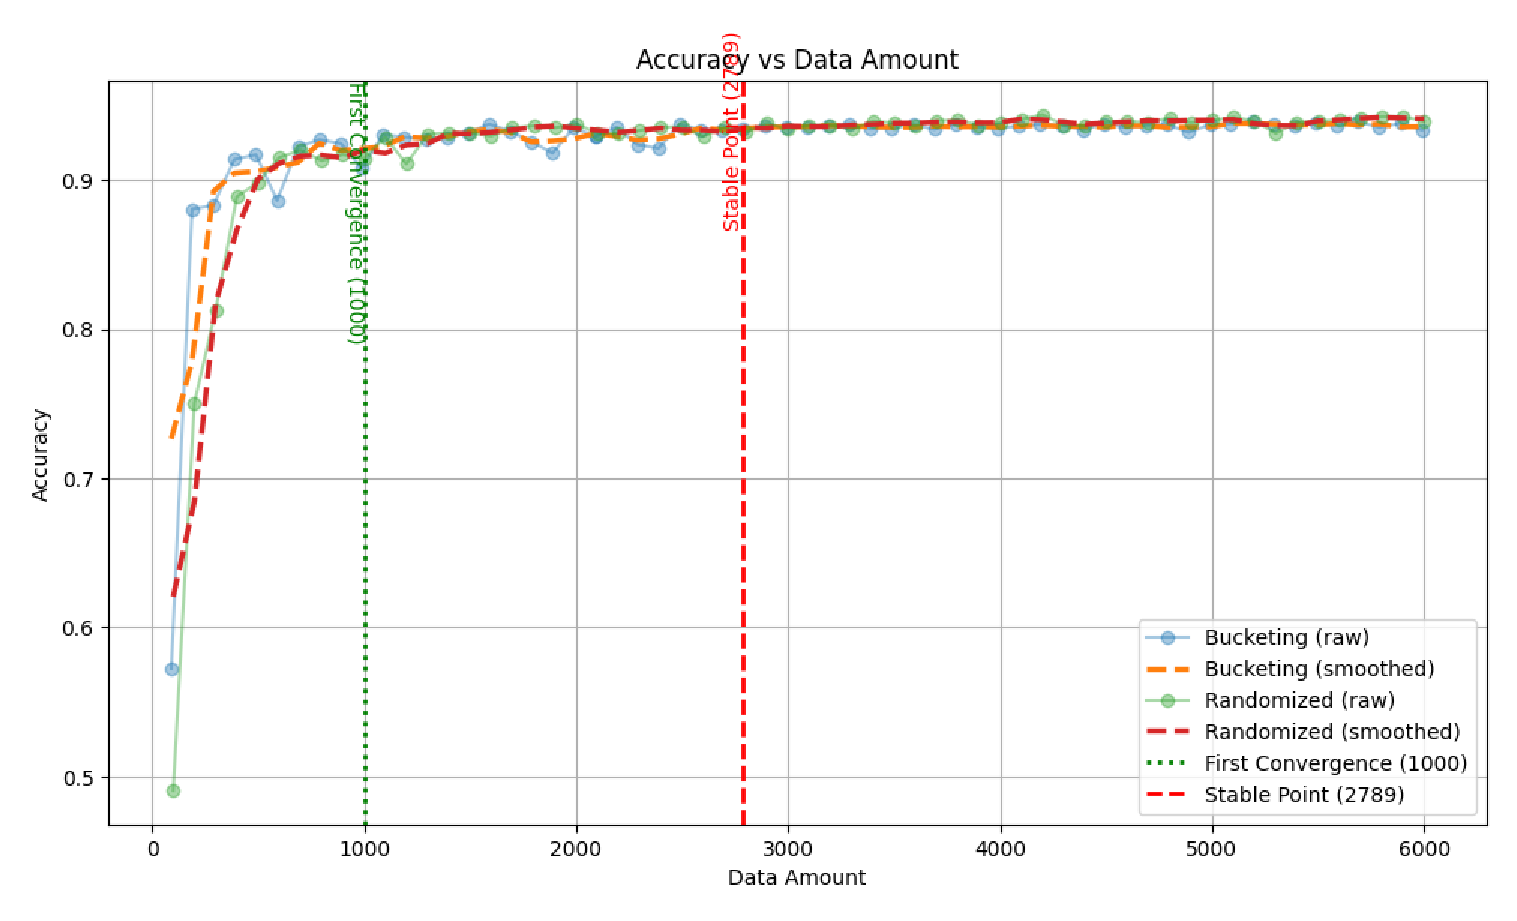
\includegraphics[width=\linewidth]{accuracy-count-2.eps}
    \caption{Evaluation Accuracy on Sample Count}
    \label{fig:accuracy-count}
\end{figure}
\indent The benefits of bucketing are further reflected in model precision (Figure \ref{fig:precision-acount}), where the bucketed model consistently outperforms the randomized model in low-sample regimes. However, unlike accuracy, precision convergence occurs much earlier—at around 689 samples. This suggests that bucketing accelerates the model’s ability to establish class boundaries and reduce false positives by providing a semantically well-structured dataset. Since precision depends only on the ratio of true positives to false positives, improvements plateau once these boundaries are learned. In contrast, accuracy, which accounts for both true positives and true negatives, requires larger sample sizes to fully converge, leading to the later stabilization observed.

\begin{figure}[H]
\centering
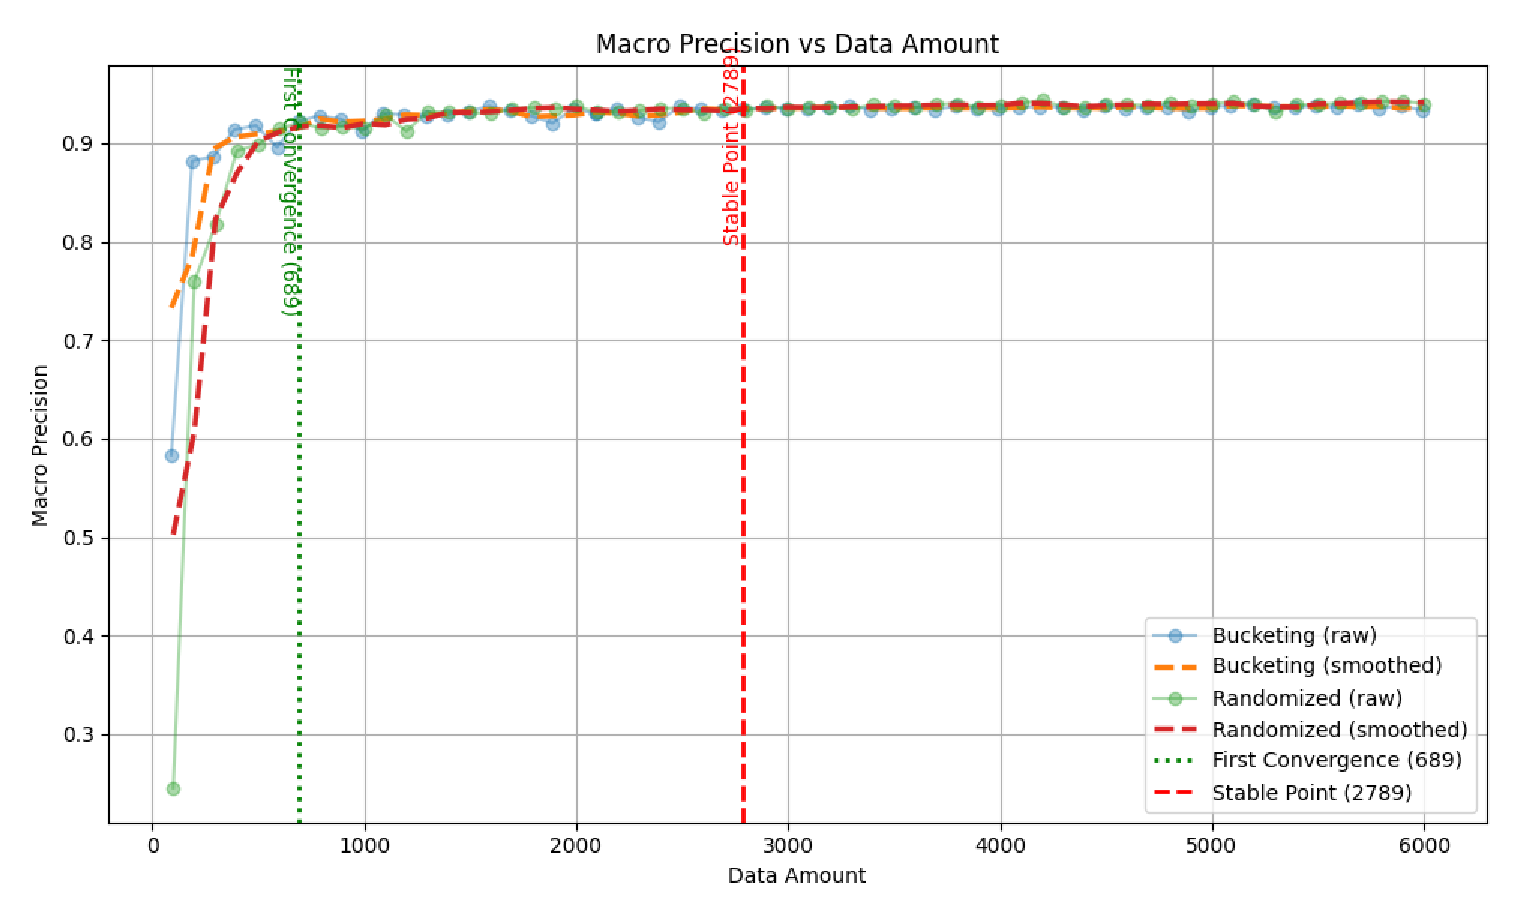
\includegraphics[width=1\linewidth]{precision-count-2.eps}
\caption{Evaluation Precision on Sample Count}
\label{fig:precision-acount}
\end{figure}

\indent Interestingly, recall converged much earlier than both precision and accuracy, stabilizing at approximately 600 samples. This indicates that the bucketed dataset enabled the model to capture a broad spectrum of positive instances with relatively few examples, thereby reducing false negatives quickly. In contrast, precision required more samples to stabilize, reflecting the additional challenge of avoiding false positives. Accuracy, which depends on both positive and negative classifications, converged latest, requiring the largest sample sizes to balance both aspects.

\subsection{Evaluation loss}
\indent Examining the overall evaluation loss of both models highlights some potential limitations of the embedding-based bucketing method. While accuracy, precision, recall, and F1 show that the bucketed model consistently outperforms the randomized model in low-sample regimes, its behavior changes as the dataset grows. As shown in Figure \ref{fig:loss-count}, the bucketed model initially achieves lower loss until approximately 490 samples, after which it experiences higher loss than the randomized model until roughly 2000 samples. This indicates that, while the bucketed model maintains comparable performance in discrete metrics, it is less confident in its predictions, assigning higher probability mass to incorrect classes.

\indent By the time the losses stabilize and converge (~2000 samples), the benefits of bucketing have largely diminished, as also reflected in the evaluation metrics (Figures \ref{fig:accuracy-count}, \ref{fig:precision-acount}, \ref{fig:recall-count}). Bucketing is designed to ensure the model sees representative examples early, but it can create “easy” and “hard” buckets. Easier buckets, containing simpler or more homogeneous samples, are learned quickly, whereas harder buckets, containing more complex or heterogeneous samples, require more data to model accurately. Since each bucket is sampled equally, this can temporarily reduce model confidence for harder samples, resulting in higher loss at intermediate dataset sizes (500 - 2000).

\indent While previous experiments focus on the effect of the implemented bucketing method on the model's performance itself, in this experiment, we will try to evaluate how effectively the implemented method separated our dataset. As previously mentioned in Section \ref{experiments:setup}, the implemented bucketing method against the \texttt{mteb/amazon\_polarity} results in 7 buckets, which includes 1 noise bucket. To properly evaluate whether the bucketing method actually created a meaningful split in the dataset, we will be training the same \texttt{bert-base-uncased} model with another bucket and then evaluating using another. The results of which will be compared to a model trained and evaluated with the same bucket (with a training and evaluation split).

\begin{figure}[H]
    \centering
    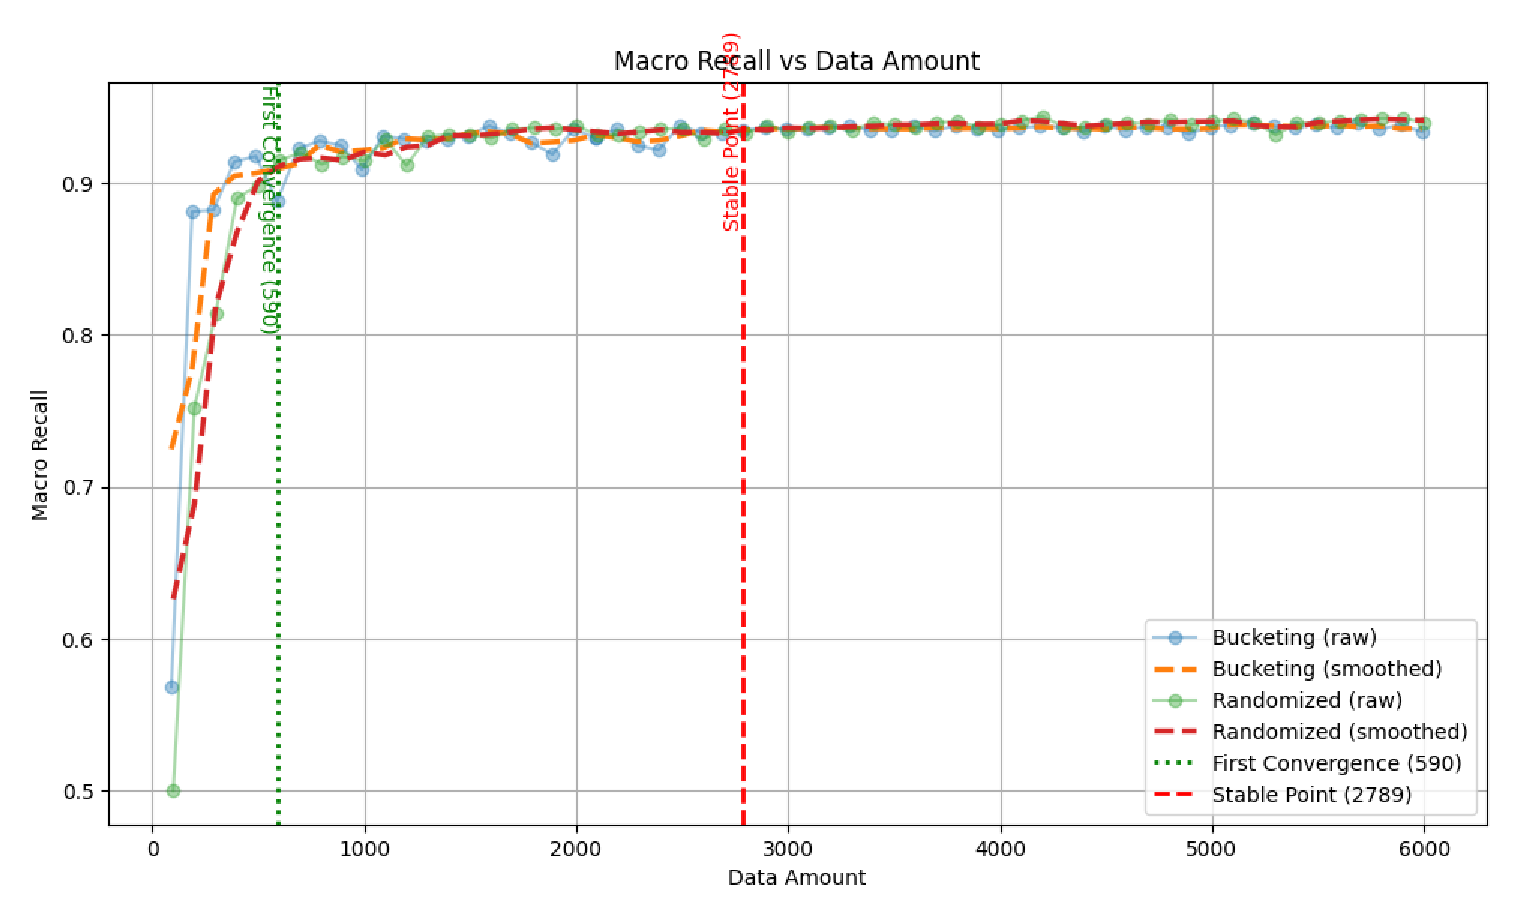
\includegraphics[width=\linewidth]{recall-count-2.eps}
    \caption{Recall on Dataset Count}
    \label{fig:recall-count}
\end{figure}

\begin{figure}[H]
    \centering
    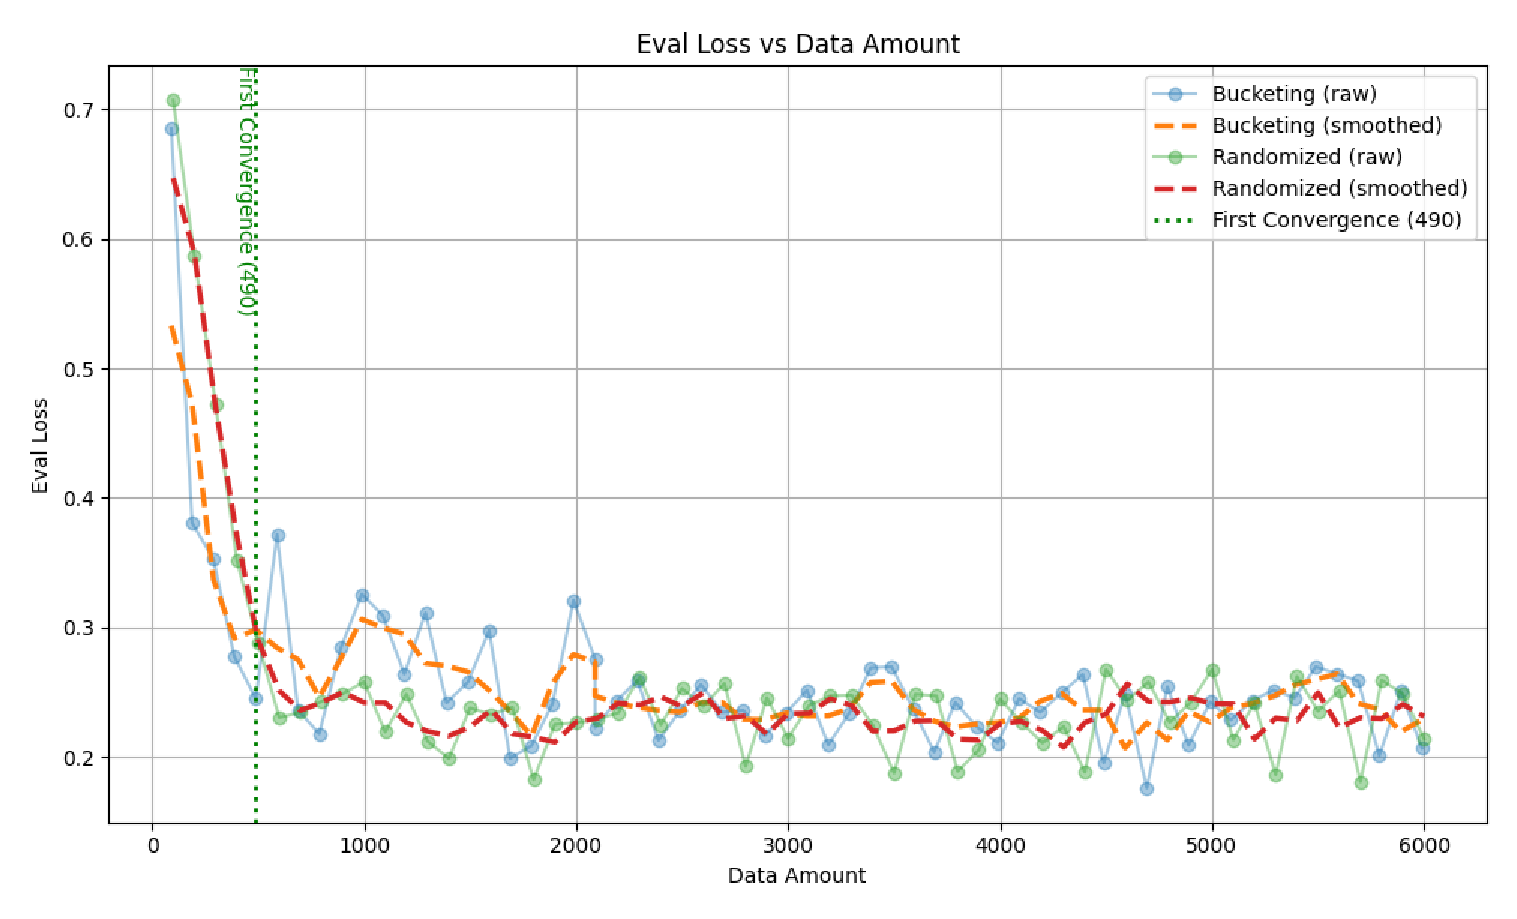
\includegraphics[width=\linewidth]{loss-count-2.eps}
    \caption{Evaluation loss On Sample Count}
    \label{fig:loss-count}
\end{figure}

\subsection{Cross-Bucket Generalization}

\indent The results of the buckets created using the previously implemented method are shown in Table \ref{tab:bucket-sizes}. The bucket with the index $-1$ represents the noise bucket, which is discarded and not used for model training. For the cross-bucket generalization experiment, we train a model on the bucket with index 4 and evaluate it on the bucket with index 2. 

\indent For comparison, we also train and evaluate a model entirely within bucket 2, using a training/evaluation split of 0.15. The hierarchical split within bucket 2 for this within-bucket experiment is summarized in Table \ref{tab:bucket2-split}.

\indent The results of the experiment can be seen in Table \ref{tab:bucket-comparison}. Although training a model on bucket 4 and evaluating it on bucket 2 still achieved relatively high performance (with higher losses), training and evaluating within the same bucket consistently produced better results across all metrics. This indicates that the implemented bucketing method successfully split the original dataset into meaningful strata, potentially allowing the model to learn more effectively from each subset and generalize better on much more heterogeneous datasets.

\section{Conclusions}\label{conclusions}
\indent This study shows promising results that embedding-based bucketing can reduce the sample size required to achieve well-performing models in extremely low-resource scenarios. Traditionally, datasets must be predetermined and manually labeled in large quantities to ensure proper generalization, which is time-consuming. By applying the semantic bucketing method, one can select representative samples from unlabeled data, potentially reducing data labeling effort while still maintaining good model generalization. Of course, any method to reduce the amount of data needed won't beat training on as much data as possible.

\begin{table}[H]
\centering
\caption{Sizes of clusters after HDBSCAN clustering. The noise bucket, containing points not assigned to any cluster, is indexed as -1.}
\label{tab:bucket-sizes}
\resizebox{0.5\linewidth}{!}{%
\begin{tabular}{c r}
\hline
\textbf{Bucket Index} & \textbf{Size} \\
\hline
-1 & 253 \\
0  & 246 \\
1  & 13,444 \\
2  & 4,767 \\
3  & 699 \\
4  & 4,841 \\
5  & 11,750 \\
\hline
\end{tabular}
}
\end{table}

\begin{table}[H]
\centering
\caption{Hierarchical Data Split for Bucket 2 (4767 samples)}
\label{tab:bucket2-split}
\resizebox{\linewidth}{!}{%
\begin{tabular}{l|c|c}
\hline
\textbf{Dataset} & \textbf{Samples} & \textbf{Percentage of Total} \\ \hline
Training Set & 3647 & 76.5\% \\
Training Evaluation (Internal Validation) & 405 & 8.5\% \\
Final Evaluation Set & 715 & 15.0\% \\ \hline
\textbf{Total} & 4767 & 100\% \\ \hline
\end{tabular}%
}
\end{table}

\begin{table}[H]
\centering
\caption{Cross-Bucket vs Within-Bucket Evaluation Metrics}
\label{tab:bucket-comparison}
\resizebox{\linewidth}{!}{%
\begin{tabular}{l|cccc}
\hline
Method & Eval Loss & Eval Accuracy & Macro F1 & Macro Precision \\ \hline
Bucket 4 → 2 & 0.2750 & 0.9287 & 0.9221 & 0.9185 \\
Bucket 2 → 2 & 0.1635 & 0.9385 & 0.9315 & 0.9274 \\ \hline
\end{tabular}%
}
\end{table}

In addition, the niche bucketing method implemented was successful in creating meaningful splits in the dataset. However, the implemented methods still remain under-researched, with open questions regarding the most optimal bucketing algorithms, hyper-parameter selection, efficiency, robustness, and reliability. As previously mentioned, different dataset characteristics may influence the overall effectiveness of the bucketing approach. Nevertheless, the implemented method may prove beneficial in other unexplored areas such as domain adaptation, few-shot learning, or cross-lingual tasks, where structured sample sampling could enhance model generalization on unseen data.

\indent This further emphasizes the need for more rigorous research before embedding-based bucketing can be considered a worthy substitute for more trusted methods such as label-based stratified sampling or embedding-size-based bucketing. Future work should explore these directions to assess whether embedding-based bucketing can mature into a reliable approach for practical applications.

\indent \textbf{Contribution.} We investigate the use of a bucketing strategy that utilizes BERT representations to construct more semantically balanced subsets for training in a low-sample environment, aiming to reduce semantic bias and lower the amount of labeled data required. To our knowledge, this specific application of embedding-based bucketing for bias mitigation in a small-sample environment has not been systematically studied.
\bibliographystyle{jplain}
\bibliography{bibliography.bib}
\end{document}